\section{Mathematik}

\subsection{Vektoren}

Darstellung:
	$\overrightarrow{a} = \mathbf{a} = \begin{bmatrix} a_1, a_2, a_3 \end{bmatrix} = \begin{bmatrix} a_1 \\ a_2 \\ a_3 \end{bmatrix}$

\begin{sectionbox}
	
	O bezeichnet den Ursprung (origo)
	
	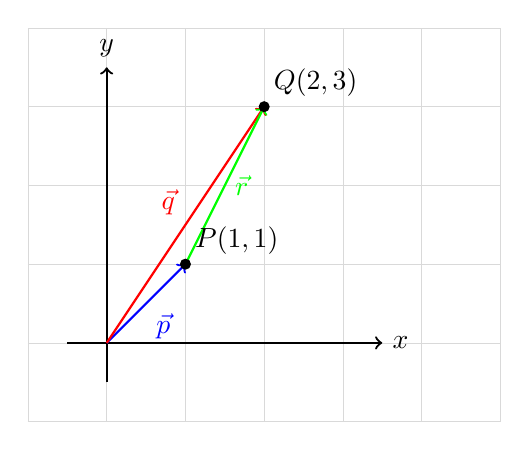
\begin{tikzpicture}
		% Draw grid
		\draw[help lines, color=gray!30] (-1,-1) grid (5,4);
		
		% Draw axes
		\draw[thick,->] (-0.5,0) -- (3.5,0) node[right] {$x$};
		\draw[thick,->] (0,-0.5) -- (0,3.5) node[above] {$y$};
		
		% Define points
		\coordinate (P) at (1,1);
		\coordinate (Q) at (2,3);
		
		% Draw vectors
		\draw[thick,->,blue] (0,0) -- (P) node[midway,below right] {$\vec{p}$};
		\draw[thick,->,red] (0,0) -- (Q) node[midway,above left] {$\vec{q}$};
		\draw[thick,->,green] (P) -- (Q) node[midway,right] {$\vec{r}$};
		% Draw and label points
		\fill (P) circle (2pt) node[above right] {$P (1,1)$};
		\fill (Q) circle (2pt) node[above right] {$Q (2,3)$};
		
	\end{tikzpicture}
	
	\begin{emphbox}
		\begin{align*}
			\overrightarrow{p} &= \overrightarrow{OP} &= \overrightarrow{P} \\
			\overrightarrow{q} &= \overrightarrow{OQ} &= \overrightarrow{Q} \\
			\overrightarrow{r} &= \overrightarrow{PQ} &= \overrightarrow{OQ} - 		\overrightarrow{OP} = \overrightarrow{q} - \overrightarrow{p}
		\end{align*}
	\end{emphbox}

	Betrag/Länge eines Vektors
	\begin{emphbox}
	\begin{align*}
		a = |\overrightarrow{a}| = \sqrt{\overrightarrow{a} {\cdot} \overrightarrow{a}} = \sqrt{a_1^2 + a_2^2 + a_3^2} 
	\end{align*}
\end{emphbox}
	
	Rechenregeln
	\begin{emphbox}
		\begin{tabular}{l|l}
			Vektoraddition/-subtraktion & 	Multiplikation mit Skalar \\
			$\overrightarrow{a} \pm \overrightarrow{b} = \begin{bmatrix} a_1 \pm b_1 \\ a_2 \pm b_2 \\ a_3 \pm b_3 \end{bmatrix} $ & $
			c {\cdot} \overrightarrow{a} = \begin{bmatrix} c {\cdot} a_1 \\ c {\cdot} a_2 \\ c {\cdot} a_3 \end{bmatrix} $ \\

			\text{Kommutativgesetz:} & $ \overrightarrow{a} + \overrightarrow{b} = \overrightarrow{b} + \overrightarrow{a} $ \\
			\text{Assoziativgesetz:} & $ (\overrightarrow{a} + \overrightarrow{b}) + \overrightarrow{c} = \overrightarrow{a} + (\overrightarrow{b} + \overrightarrow{c}) $ \\
			\text{Distributivgesetz:} & $ \lambda {\cdot} (\overrightarrow{a} + \overrightarrow{b}) = \lambda {\cdot} \overrightarrow{a} + \lambda {\cdot} \overrightarrow{b} $
		\end{tabular}
	\end{emphbox}

	Einheitsvektor \\
	- markiert mit Zirkumflex \\
	- Zeigt in gleiche Richtung, aber mit Länge 1
	\begin{emphbox}
		\begin{align*}
	 		\hat{a} &= \frac{1}{|\overrightarrow{a}|} {\cdot} \overrightarrow{a} \\
	 		|\hat{a}| &= 1
		\end{align*}
	\end{emphbox}

	
	Normalenvektor

	Steht orthogonal auf einer Geraden, Kurve oder Ebene

	Normaleneinheitsvektor
	
	Normalenvektor mit Länge 1.
	
	\begin{emphbox}
		\begin{align*}
			\overrightarrow{n_0} = \frac{1}{|\overrightarrow{n}|} {\cdot} \overrightarrow{n} \text{Vektor mit Richtung von a, mit Länge 1}
		\end{align*}
	\end{emphbox}
	mit: $\overrightarrow{n_0}$: Normaleneinheitsvektor, $\overrightarrow{n}$: Normalenvektor

	Nullvektor
	Richtung undefiniert, Länge = 0

\end{sectionbox}
\begin{sectionbox}
	Skalarprodukt (Punktprodukt, inneres Produkt)
	\begin{emphbox}
		\begin{tabular}{lcl}
			\text{Geom. Form:} & $ \overrightarrow{a} {\cdot} \overrightarrow{b} $ & $ = \lvert \overrightarrow{a} \rvert {\cdot} |\overrightarrow{b}| {\cdot} \cos \alpha $ \\

			\text{Koord.form:} & $ \overrightarrow{a} {\cdot} \overrightarrow{b} $ &= $ \begin{bmatrix} a_1 \\ a_2 \\ a_3 \end{bmatrix} {\cdot} \begin{bmatrix} b_1 \\ b_2 \\ b_3 \end{bmatrix} = a_1 {\cdot} b_1 + a_2 {\cdot} b_2 + a_3 {\cdot} b_3 $ \\

			\text{...} & $ \overrightarrow{a} \perp \overrightarrow{b}$ & $\Leftrightarrow \overrightarrow{a} {\cdot} \overrightarrow{b} = 0 $ \\

			\text{Kommutativgesetz:} & $ \overrightarrow{a} {\cdot} \overrightarrow{b}$ &= $\overrightarrow{b} {\cdot} \overrightarrow{a}$ \\

			\text{Assoziativgesetz:} & $(\lambda {\cdot} \overrightarrow{a}) {\cdot} \overrightarrow{b}$ &= $\lambda {\cdot} (\overrightarrow{a} {\cdot} \overrightarrow{b})$ \\

			\text{Distributivgesetz:} &	$\overrightarrow{a} {\cdot} (\overrightarrow{b} + \overrightarrow{c})$ &= $\overrightarrow{a} {\cdot} \overrightarrow{b} + \overrightarrow{a} {\cdot} \overrightarrow{c}$
		\end{tabular}
	\end{emphbox}

	Kreuzprodukt (Vektorprodukt, äusseres Produkt)
	\begin{emphbox}
		\begin{tabular}{lcl}
			\text{Geom. Form:} & 
			$\overrightarrow{a} \times \overrightarrow{b}$ &= $|\overrightarrow{a}| {\cdot} |\overrightarrow{b}| {\cdot} \sin \alpha
			{\cdot} \overrightarrow{n}$ \\

			\text{Koord.form:} & $\overrightarrow{a} \times \overrightarrow{b}$ &= $\begin{bmatrix} a_1 \\ a_2 \\ a_3 \end{bmatrix} \times \begin{bmatrix} b_1 \\ b_2 \\ b_3 \end{bmatrix} = \begin{bmatrix} a_2 {\cdot} b_3 - a_3 {\cdot} b_2 \\ a_3 {\cdot} b_1 - a_1 {\cdot} b_3 \\ a_1 {\cdot} b_2 - a_2 {\cdot} b_1 \end{bmatrix}$ \\

			\text{nicht kommutativ!:} &	$\overrightarrow{a} \times \overrightarrow{b}$ & $= -(\overrightarrow{b} \times \overrightarrow{a})$ \\

			\text{Distributivgesetz:} &	$\overrightarrow{a} \times (\overrightarrow{b} + \overrightarrow{c})$ &= $\overrightarrow{a} \times \overrightarrow{b} + \overrightarrow{a} \times \overrightarrow{c}$ \\

			\text{Alt. Schreibweisen:} & $\overrightarrow{a} \times \overrightarrow{b}$ & $\equiv \overrightarrow{a} \wedge \overrightarrow{b} \equiv	[\overrightarrow{a}, \overrightarrow{b}]$
		\end{tabular}
		
	\end{emphbox}
	mit: $\overrightarrow{n}$: Einheitsvektor senkrecht zu $\overrightarrow{a}$ und $\overrightarrow{b}$
	Kreuzprodukt bildet ein Rechtssystem. Rechte-Hand-Regel: x: Daumen, y: Zeigefinger (abgespreizt), z: Mittelfinger

%	\begin{emphbox}
%	\begin{align*}
%		\text{mit: \overrightarrow{n}: Einheitsvektor senkrecht zu \overrightarrow{a} und \overrightarrow{b} }
%		\end{align*}
%	\end{emphbox}
	
\end{sectionbox}
